\chapter{Physikalische Gr"o"sen}

\begin{Def}[Physikalische Gr"o"se]\index{Gr"o"se}\index{Physikalische Gr"o"se}
   besteht stets aus
     $$
     <\text{Zahlenwert}> \cdot <\text{Einheit}>
     $$
\end{Def}
Man versucht sich dabei auf m"oglichst wenige Einheiten -- die
sog. \textbf{Basiseinheiten} -- zu beschr"anken.
\begin{Def}[Basiseinheit/Grundeinheit]\index{Basiseinheit}
   Grundlage f"ur Physkalische Gr"o"sen und Messwerte; m"ussen "uberall
   bestimmbar bzw. nachpr"ufbar sein und orientieren sich deshalb oft
   an Naturkonstanten.
\end{Def}

\begin{Beispiel}
 Der \emph{in} wurde ursprünglich definiert als Breite des Daumens des 
damaligen Königs.  Doch ist diese Einheit nicht nachprüfbar, deshalb wurde 
der \emph{in} später umdefiniert als die Länge von insgesamt drei Gerstenkörner.

Man hat den Wunsch nach Basiseinheiten.
\end{Beispiel}








\section{Basiseinheiten}



\subsection{Vorsilben}

Zehnerpotenzen der Form $10^{3k}$ werden bei Physikalischen Gr"o"sen durch
\emph{Vorsilben} vor den Einheiten ersetzt:
\begin{center}
% use packages: array
\begin{tabular}{c l c}
\toprule
 Zehnerpotenz & Vorsilbe & Abk"urzung \\
 \midrule
-18 & atto & a\\ 
-15 & fempto & f \\ 
-12 & pico & p  \\
-9  & nano & n  \\
-6  & micro & $\mu$  \\
-3 & milli & m  \\
0  & -- & --  \\
3  & Kilo& K  \\
6  & Mega & M  \\
9  & Giga & G  \\
12 & Terra & T \\
\bottomrule
\end{tabular}
\end{center}







\subsection{Zeit}

\begin{Def}[Sekunde \textbf s]\index{Sekunde}\label{def_sekunde}
   $1s = 9 \, 192\, 631\, 770 \cdot T_A$, wobei $T_A$ die
   Periodendauer des Hyperfein"ubergangs von $^{133}Cs$ ist -- ein sehr
   pr"azise stattfindender Vorgang in C"asiumatomen.
\end{Def}

Um \textbf{sehr kurze} Zetr"aume zu messen, verwendet man schwingende
Quarze oder andere periodische Vorg"ange in Atom(kern)en. F"ur
\textbf{sehr lange} Zeitr"aume dagegen verwendet man bspw. radioaktiv
zerfallende Stoffe und deren Halbwertszeit.

 \begin{table}[ht]
 \begin{tabular}{l r}
 Existenz des Weltalls: & $10^{18} $s \\
 Lebensdauer eines Menschen: & 1$10^9 $s \\
 Pulsschlag: & $1 $s \\
 Licht durchläuft $30 cm$: & $10^-9 $s \\
 Licht durchläuft Atom: & $10^-18 $s
 \end{tabular}
\caption{Größenordnung von Zeiten}
 \end{table}

\begin{Beispiel}
\begin{itemize}
\item Ein Federpendel ist für kleine Auslenkwinkel, annähernd harmonisch.  Für \emph{harmonische Schwingungen} gilt für die Periodendauer $T$:
\[
\boxed{T=2\pi \sqrt{\frac{l}{g}}}
\]
So lässt sich die Sekunde beispielsweise definieren als die  Dauer für eine Schwingung des Federpendels der Länge $l=24,8 \text{cm}$.
\item Quarzplättchen besitzen eine Frequenz aus dem $kHz$-Bereich.
% \begin{figure}
% 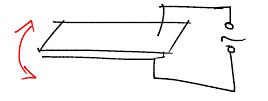
\includegraphics[scale=0.5]{fig5.png}
% \end{figure}

Sie Besitzen einen Gangungenauigkeit von $1$ s/Woche. Sie besitzen also einen Fehler von $1$s pro $10^6$s
\item Es gibt aber auch die Möglichkeit mittels atomarer Eigenschwingungen (atomare Uhren) die Zeit noch genauer zu messen.  Deren Ganggenauigkeit entspricht $1$ s/$3000$ Jahren. Dies findet unter anderem Anwendung im GPS. 
\item $\ce{^{133}Cs}$ Hyperfeinübergang

Es ergibt sich die Definition $1\s=9.192.631.770$-faches der Periodendauer des Hyperfeinübergangs in $\ce{^{133}Cs}$. Diese ist überall nachvollziehbar!
\item Zeitmessung durch radioaktiven Zerfall Kerne mit großer Masse $\rightarrow$ instabil $N=$ Zahl instabiler Kerne. \\

Es gilt die Proportionalität $\frac{dN(t)}{dt} \sim N(t) $, dabei zerfallen die Kerne unabhängig voneinander. ($\rightarrow$ \emph{Unabhängigkeit}) 

 \begin{equation*}
  \frac{dN}{dt}=-\lambda \cdot N(t), \qquad \lambda: \text{ Zerfallskonstanste}, \lambda>0
 \end{equation*}
 \begin{equation*}
  N(T)=N_0 \cdot e^{-\lambda t}, \qquad N_0:= N(0), [\lambda]=\frac{1}{s}
 \end{equation*}

  \begin{figure}[ht]
   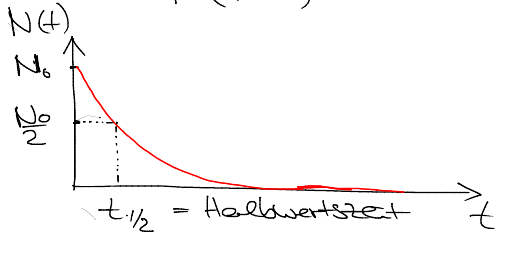
\includegraphics[scale=0.5]{bilder/fig6}
  \end{figure}

\begin{align*}
  \frac{N_0}{2} &= N_0 \cdot e^{-\lambda t_{\frac 1 2}}\\
  \ln 0.5 &=-\lambda \cdot t_{\frac 1 2} \\
  t_{\frac 1 2} &= - \frac{\ln 0.5}\lambda = {\ln 2}{\lambda} 
\end{align*}

 \begin{ex*}
  \begin{enumerate}[a)]
   \item $\ce{^{224}_{88} Tn} \rightarrow \ce{^{220}_{86} Ru} + \alpha, \qquad \alpha=\ce{^4_2 He}$ mit Halbwertszeit $t_{\frac 1 2}=556s$
   \item $\beta$-Zerfall: $\ce{^{14}_6 C} \to \ce{^{14}_7 N} + e^- \bar v_l$ mit Halbwertszeit $t_{\frac 1 2}=5730 a$  
 \end{enumerate}
 \end{ex*}
\item Radio-Carbon-Methode \\
 Kohlenstoff liegt in der Athmosphäre in den Isotopen $\ce{^{12}_6 C}, \ce{^{13}_6 C}, \ce{^{14}_6 C}$ vor.

\begin{table}
\centering
 \caption{Verteilung in Atmosphäre}
 \begin{tabular}{c|c}
  $\ce{^{12} C}$&  $98,89\%$ \\
  $\ce{^{13} C}$& $1,11\%$ \\
 $\ce{^{14} C}$& $10^-10 \%$ \\
 \end{tabular}
\end{table}
 Wobei erstere beiden stabil und $\ce{^{14} C}$ instabil ist.  Lebende Organismen besitzen aufgrund von Stoffaustausch identische Kohlenstoff-Verteilung.  Stirbt der Organismus verändert sich das Isotopenverhältnis.

 
 \begin{align*}
  \ce{^{14} C(t)}&=\ce{^{14} C_0} \cdot e^{-\lambda t} \\
 \ce{^{13} C(t)}&=\ce{^{12} C_0}\\
 \frac{\ce{^{14} C}}{\ce{^{12} C}} |_\text{Fossil} (t)&= \frac{\ce{^{14} C_0}}{\ce{^{12} C_0}} e^{-\lambda t}, \qquad \lambda=1.121\cdot 10^{-4} \frac{1}{a}
 \end{align*}
\item C14-Methode: experimentelle Bestimmung\\
Die Zerfalleigenschaft des $C-14$, lässt sich ausnutzen, um kleine Zeitmaße zu messen.
\begin{ex*}
 $\frac{\ce{^{14}  C}}{\ce{^{12} C}}$ im Fossil (Massenspektrum) $\rightarrow$ Alter $t \rightarrow$ Alter + Höhlenzeichnung in S-Frankreich:  $15.500$ Jahre
\end{ex*}
\end{itemize}
\end{Beispiel}





\subsection{L"ange}

\begin{Def}[Meter \textbf m]\index{Meter}\label{def_meter}
   $1m = c_0 \cdot \frac{1}{299\, 792\, 458}\operatorname{s}$ mit der
   (Vakuum)Lichtgeschwindigkeit $c_0$.
\end{Def}

Um \textbf{sehr gro"se} Abst"ande zu messen, benutzt man
Triangulationsverfahren. Bei \textbf{sehr kleinen} Abst"anden
Laserinterferomenter, bei denen man ausnutzt, dass sich Lichtwellen
bei bestimmten Bedingungen ausl"oschen und die Lichtwellenl"ange bekannt
ist.

\begin{table}[ht]
\centering
\caption{Größenordnung von Längen}
 \begin{tabular}{l r}
  Erde-Fixstern & $4\cdot 10^{16} \m$\\
  Erde-Sonne & $1.5 \cdot 10^{11} \m$\\
 Erdradius & $63 \cdot 10^6 \m $\\
 Sichtbares Licht (Wellenlänge) & $ 500\cdot 10^{-9}$m \\
 Atomdurchmesser & $10^{-10}$m  \\
 Kerndurchmesser & $10 ^{-15}$m
 \end{tabular}
 \end{table}
 \newpage
\begin{Beispiel}
\begin{itemize}
\item Geschichte des Meters:\\
1799 wurde der Meter definiert durch $1 \m \hat = \frac{1}{400000000}$ des durch Paris gehenden Großkreises ($40\cdot 10^3$ km). 1795 wurde ein Prototyp des Urmeters aus Messing hergestellt.

Einige Jahre später wurde der Urmeter aus Platin hergestellt und in einem Stahlschrank im französischen Nationalarchiv 1799 verschlossen. Heute wird es in einem Tresor des Internationalen Büros für Maße und Gewicht (BIPM) in S\`evres aufbewahrt.

1889 wurde das Urmeter von der Generalkonferenz für Maß und Gewicht durch das Urmeter einer Platinlegierung($90\% \ce{Pt}$ und $10\% \ce{Ir}$) ersetzt.

 Seit 1983 ist der Meter über den Lichtweg definiert:
 \[
  1\m=\text{ Länge des Weges Weges, den Licht im Vakuum in $\frac{1}{299792485} s$ zurücklegt.}
 \]

\item Messung von Abständen mittels Triangulation:\\
 \begin{figure}[!ht]
  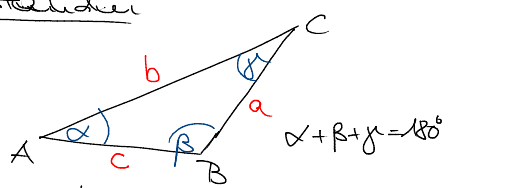
\includegraphics[scale=0.5]{bilder/fig7}
 \end{figure}
 Sinussatz: $\frac{c}{\sin\gamma} = \frac{a}{\sin{\beta}}=\frac{a}{\sin\alpha}$ \\
 
 \begin{itemize}
  \item $\alpha, \beta$ bekannt $\to \gamma$ bekannt
  \item $c$ bekannt, dann lässt sich $a$ bzw. $b$ berechnen zu:
\begin{align*}
a&=c\cdot \frac{\sin \alpha}{\sin \gamma}\\
b&=c\cdot \frac{\sin \beta}{\sin \gamma}
\end{align*}
 \end{itemize}
\newpage
\item Abstand-Erde-Mond \\
 \begin{figure}[!h]
  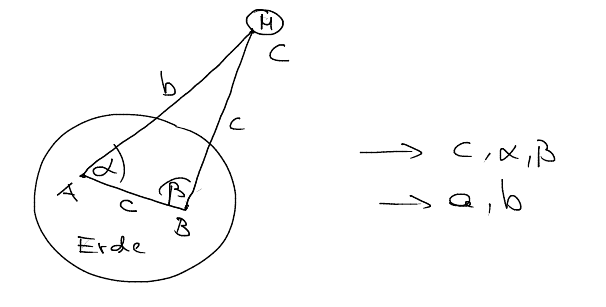
\includegraphics[scale=0.5]{bilder/fig8}
 \end{figure}

\item Abstand Erde-Sonne\\
 Als Basis (c) wähle Erde-Mond
 \begin{figure}[!h]
  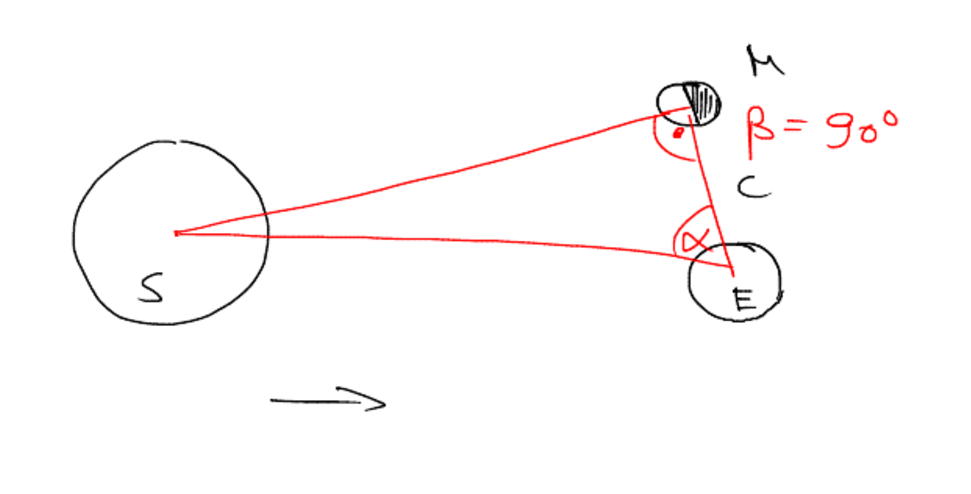
\includegraphics[scale=0.5]{bilder/fig9}
 \end{figure}
 Bei Halbmond besitzt $\beta=90^\circ$.  Den Abstand Erde-Mond lässt sich messen. Dann genügt es Den Winkel zwischen Mond und Sonne auf der Erde messen und damit ergibt sich der Abstand zum Mond.

\item LIDAR (Light Detection and raging)\\
 \begin{figure}[!h]
  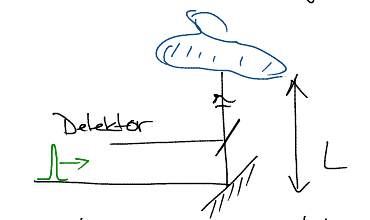
\includegraphics[scale=0.5]{bilder/fig10}
 \end{figure}
 \[
 T=\frac{2L}{c}
 \]
 
\item Messungen kleiner Entfernungen Laserinterferometer (\emph{Michelson-Interferometer})

%  \begin{figure}[ht]
%   \includegraphics[scale=0.7]{fig11}
%  \end{figure}

 \[
  \Delta s= 2 |s_1-s_2|
 \]

 Die Verschiebung um $\frac{20 \my m}{\text{64 Maxima}}=0.625 \to \lambda=630\my \m $
\end{itemize}
\end{Beispiel}




\subsection{Masse}

\begin{Def}[Kilogramm
   \textbf{Kg}]\index{Kilogramm}\label{def_kilogramm}
   $1Kg = \text{Masse des Urkilogramms}$. Das Urkilogramm ist ein
   Gewicht in Paris, welches das Kilogramm definiert.
\end{Def}

Das Kilogramm ist also eine \emph{willk"urliche} {Definition} und nicht
"uber Natukrkonstanten definiert. Man versucht hier Abhilfe zu
schaffen, indem man bspw. eine monokirstalline Siliciumkugel erstellt,
bei der man genau die Anzahl der Atome bestimmen kann, deren einzelnes
Gewicht bekannt ist -- so k"onnte man eine allgemeine, (unter gro"sem
Aufwand) reproduzierbaer Definition des Kilogramms erstellen.







\subsection{MKS-System}
\label{kap_mks-system}

\begin{Def}[MKS-System]\index{MKS-System}
   Ein \emph{Ma"ssystem}, welches alle in der \emph{Mechanik} wichtigen
   Einheiten auf die drei Grundeinheiten
   \begin{itemize}
   \item Meter
   \item Kilogramm
   \item Sekunde
   \end{itemize}
   zur"uckf"uhrt.
\end{Def}

\index{SI-System} Das \textbf{SI-System} (\emph{System
  Internationale}) stellt dar"uber hinaus weitere Einheiten zur
Verf"ugung, die Grundlage sind f"ur weitere Teilgebiete der Physik:

\begin{description}[\setlabelstyle{\bfseries\slshape}]
\item[Thermodynamik] Absolute Temperatur in Kelvin $\mathbf
   K$\\Stoffmenge in Mol $\mathbf{mol}$
     \item[Elektrodynamik] Stromst"arke in Ampere $\mathbf A$
     \item[Optik] Lichtst"arke in Candela $\mathbf{Cd}$
 \end{description}






\section{Messfehler}\index{Messfehler}

\subsection{Systematischer Messfehler}

\begin{Def}[Systematischer Messfehler]\index{Systematischer
     Messfehler}
     Als \emph{systematischer Fehler} (auch systematische Abweichung oder -Verzerrung; engl. systematic error oder bias) werden in der Technik, den Natur- und anderen Wissenschaften Messfehler bezeichnet, die sich bei wiederholter Messung nicht im Mittel aufheben. Diese Fehler sind prinzipiell vermeidbar.
\end{Def}

\textbf{Ursachen} k"onnen sein:
\begin{itemize}
     \item ein falsch geeichtes Messinstrument
     \item Nichtberücksichtigen von \emph{Konstanten} äußerer Einflüsse
     \item Rundungen / Vereinfachungen in den Formeln (zum Beispiel die Anwendung der Kleinwinkelnäherungen $ \sin \alpha \approx \alpha $ und $ \cos \alpha \approx 1 $
\end{itemize}




\subsection{Statistische (zuf"allige) Messfehler}

\begin{Def}[Statistische Messfehler]\index{Statistische Messfehler}
   Als \emph{zufällige Abweichungen} oder \emph{Zufallsfehler} werden die Abweichungen der Messwerte von ihrem Mittelwert bezeichnet. 
   Zufällige Abweichungen streuen in Betrag und Vorzeichen. Sie sind im Allgemeinen nicht vermeidbar.
\end{Def}

\textbf{Ursachen} k"onnen sein:
\begin{itemize}
     \item Ablesefehler durch Beobachter (wobei diese natürlich auch systematisch sein können, durchaus sind aber auch Streuungen beim Ablesen denkbar)
     \item (statistische) Schwankungen "au"serer Einfl"usse
\end{itemize}

Diese Fehler sind i.A. nicht vermeidbar, jedoch verringerbar. Man
bedient sich dazu statistischer
Auswertungsmethoden\index{Statistik}. Wiederholt man den Versuch oft,
kann man einen \textbf{Mittelwert}
\begin{equation}
     \bar x = \frac{1}{n} \cdot \sum_i x_i
\end{equation}
der $n$ Messwerte $x_i$ bestimmen. 

Weiter gibt die \textbf{Standardabweichung} oder \textbf{Streuung}
\begin{equation}
     \sigma = \sqrt{\frac{1}{n-1} \cdot \sum_i (x_i - \bar x )^2}
\end{equation}
an, wie zuverl"assig $\bar x$ ist -- Messwerte $x_i$ innerhalb der
$\sigma$-Umgebung von $\bar x$ treten mehr als halb so h"aufig auf, wie
$\bar x$ selbst.

Um die W"ahrscheinlichkeit $p$ zu berechnen, mit der ein bestimmter
Messwert $x$ auftreten sollte, verwendet man die
\textsc{Gauss}'sche-Normalverteilung\index{Normalverteilung}. Diese besitzt die Wahrscheinlichkeitsdichte:
\begin{equation}
   p(x) = \frac{1}{\sqrt{2\pi} \cdot \sigma} \cdot 
   \exp\left ( \frac{- (x-\bar x)^2}{2\sigma^2} \right )
\end{equation}
Als Dichtefunktion besitzt $ p $ die Eigenschaft:
\[
P(]-\infty, \infty[)=\int_{-\infty}^{\infty} p(x)\, dx=1
\]

\subsection{Exkurs: Wahrscheinlichkeitstheorie $ (\bigstar) $}
\begin{Def}[Wahrscheinlichkeitstheorie aus WIKIPEDIA]
Die Wahrscheinlichkeitstheorie oder Wahrscheinlichkeitsrechnung ist ein Teilgebiet der Mathematik, das aus der Formalisierung der Modellierung und der Untersuchung von Zufallsgeschehen hervorgegangen ist. Gemeinsam mit der mathematischen Statistik, die anhand von Beobachtungen zufälliger Vorgänge Aussagen über das zugrunde liegende Modell trifft, bildet sie das mathematische Teilgebiet der Stochastik. Die zentralen Objekte der Wahrscheinlichkeitstheorie sind zufällige Ereignisse, Zufallsvariablen und stochastische Prozesse.
\end{Def}
Im Folgenden möchten wir einige wahrscheinlichkeitstheoretische Begriffe kurz erklären. 
\begin{description}
\item[Wahrscheinlichkeit:] Die Wahrscheinlichkeit (Probabilität) ist eine Einstufung von Aussagen und Urteilen nach dem Grad der Gewissheit (Sicherheit). Im Zusammenhang mit der Maßtheorie bezeichnen wir ein Maß $ P $ als Wahrscheinlichkeitsmaß, ein Maß, dass in seiner Gesamtheit ihrer Ereignisse 1 ist.
\item[Maß:] Wir bezeichnen $ \my: C \to [0, \infty] $ mit $ A_i \in C $, wobei $ C $ die Menge der möglichen Ereignisse bezeichnet, als Maß falls gilt:
\begin{itemize}
\item $ \my(\emptyset)=0 $
\item  $ \sigma- $Additivität: $ \my\left ( \bigcup_{i\ge 1} A_i \right )= \sum_{i\ge 1} \my(A_i) $
\end{itemize}
\item[Verteilungsdichte:] Mittels der Verteilungsdichte $ f $ können wir die Wahrscheinlichkeit des Ereignisses berechnen durch:
\[
P([a,b])=\int_a^b f(x) \, dx
\]
Bestimmte Verteilungsarten (z.B.: unitäre (bedeutet: gleichverteilt) Verteilung, Normal-/GAUSS-Verteilung)
\item[Verteilungsfunktion:] Auch die Verteilungsdichte $ F $ ermöglicht uns die Berechnung der Wahrscheinlichkeit
\[
P([a,b])=F(b)-F(a)
\]
Die Verteilungsfunktion hat einige Grundlegende,  sie wächst monoton und ist rechtsseitig stetig. Dies liegt natürlich nahe, da es sonst negative Wahrscheinlichkeiten gäbe. Auch diese hängen von der Art der Verteilung (dies entspricht im Wesentliche die Art des Zufalls) ab.
\item[Zähldichte] Ist die Grundmenge der Ereignisse endlich, so bezeichnen wir den Wahrscheinlichkeitsraum als diskret (so zum Beispiel beim Münzwurf oder Würfel). In diesem Fall,  können wir für die Einzelergebnisse Wahrscheinlichkeiten angeben wir bezeichnen die Zugehörige Funktion $ f $ als Zähldichte. Es gilt:
\[
P(\{x\})=f(x)
\]
\item[Unabhängigkeit] Wir sagen zwei Ereignisse $ A, B $ sind unabhängig, wenn gilt:
\[
P(A\cap B)=P(A)\cdot P(B)
\]
Dies entspricht der Baumregel für diskrete Wahrscheinlichkeitsräume.  Also, sind Ereignisse unabhängig, wenn die Messungen nicht voneinander abhängen, also in keiner Relation zueinander sind. Ein Beispiel wäre das Würfeln mit zwei Würfeln. 
\end{description}

\begin{Wichtig}
Weder bedeutet Wahrscheinlichkeit 0, dass ein Ergebnis nicht eintreffen kann, noch sagt die Wahrscheinlichkeit 1, dass das Ergebnis stets eintrifft. Dies kann man sich daran verdeutlichen, dass es "`unendlich"' unwahrscheinlich, dass wenn man von einem Hochhaus einen Stein runterwirft, ihn exakt an einem gewissen Punkt wiederzufinden, jedoch kann tatsächlich jeder beliebige Punkt (zu mindest theoretisch) erreicht werden. Dagegen ist es "`unendlich"' wahrscheinlich, dass der Stein außerhalb des Punkts aufkommt, doch auch dies ist natürlich nicht notwendigerweise der Fall.  Für Wahrscheinlichkeit 1 sprechen wir von einer $ P $-fast sicheren Eigenschaft.  
\end{Wichtig}









